\subsubsection{Use Case}
Here follows the use case diagram: \\

\begin{figure}[H]
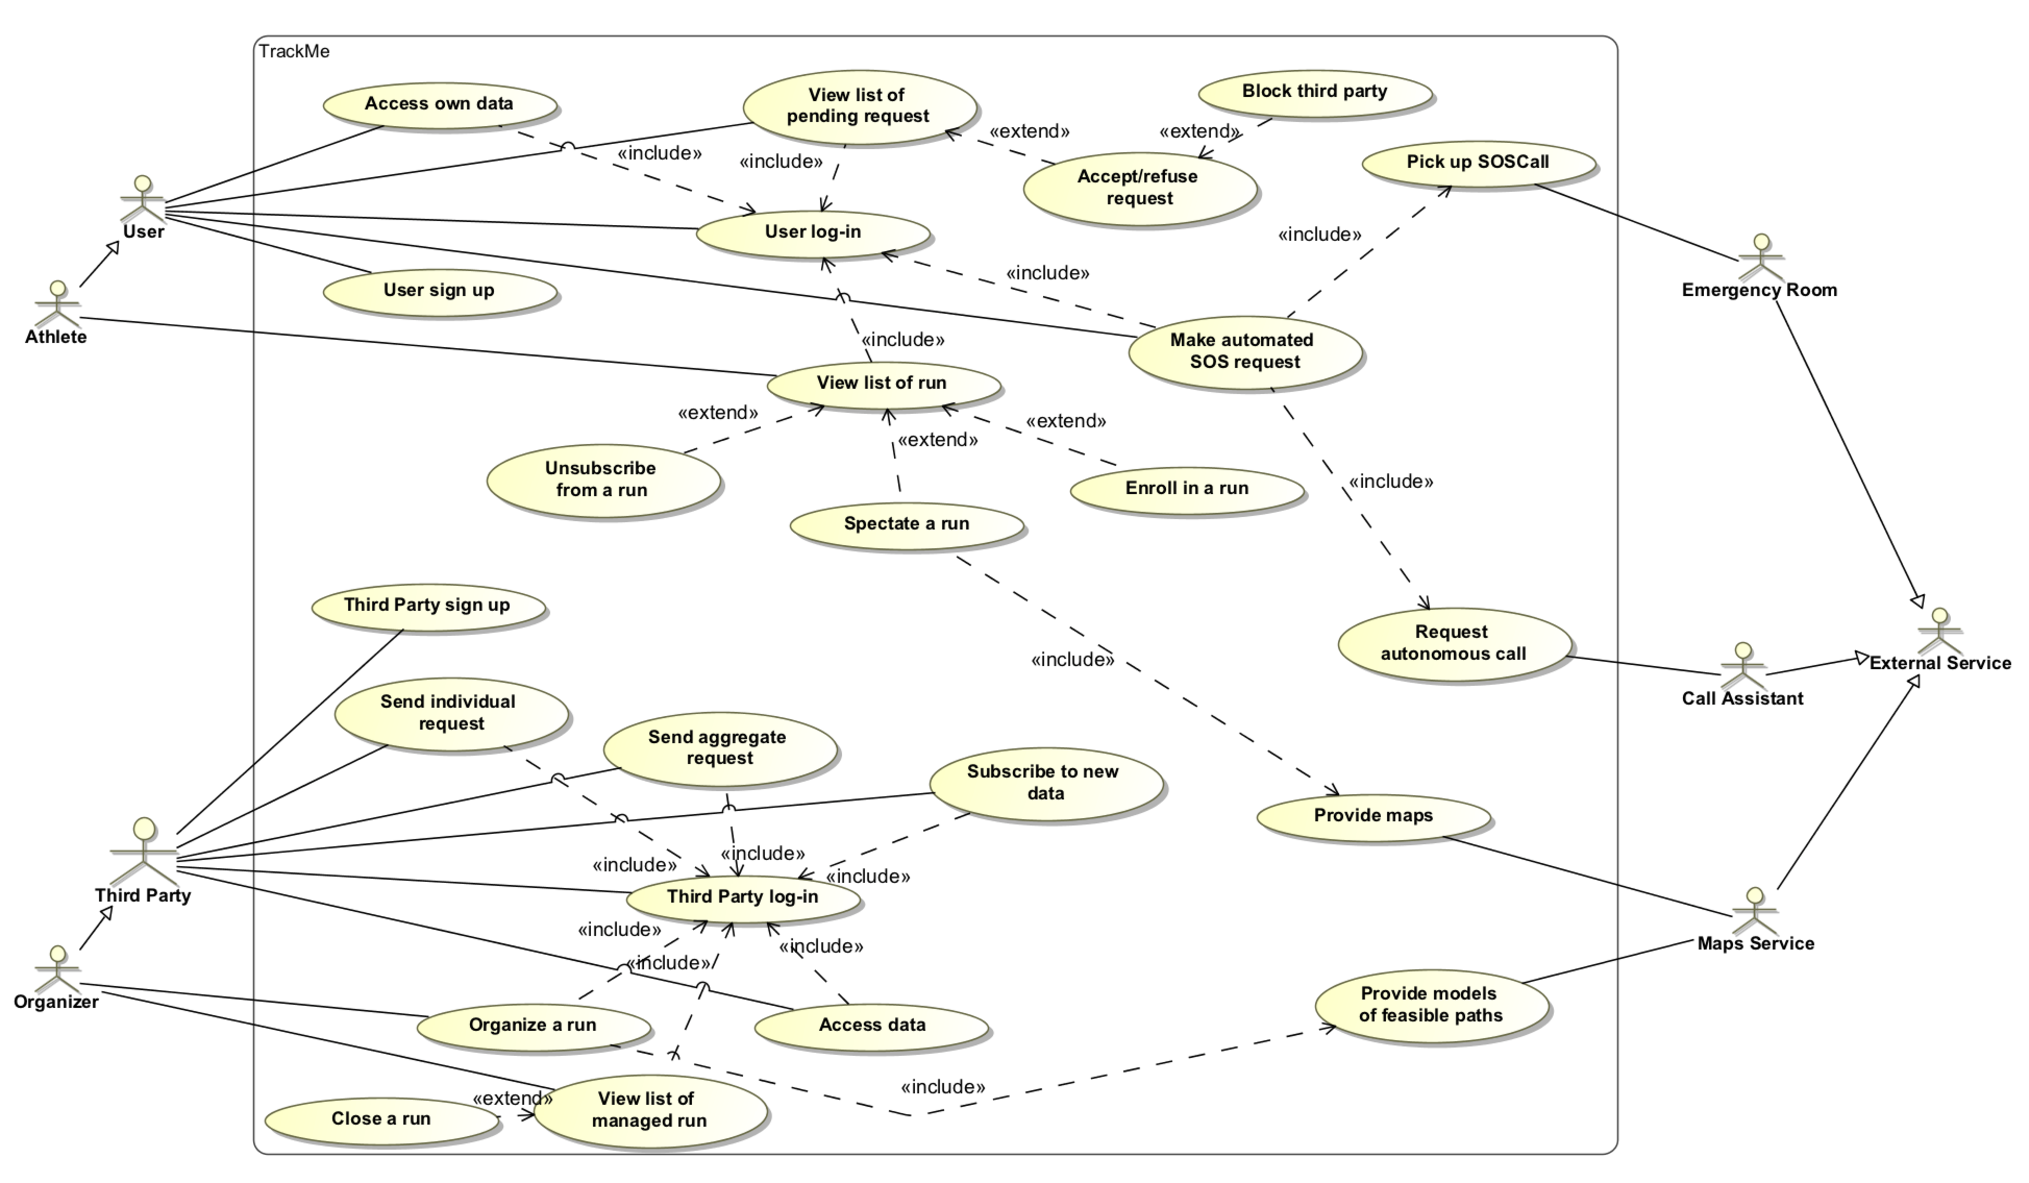
\includegraphics[width=\linewidth]{Images/usecase}
\caption{Use case diagram}
\label{fig:usecasediagram}
\end{figure}

\par 
Beneath, the use case are analyzed:	\\

\begin{table}[H]
\begin{tabularx}{\textwidth}{|l|X|}
\hline
 Name & Send aggregated request \\ \hline
 Actor & Third party customer  \\ \hline
 Entry conditions & Third party customer needs some aggregated data on anonymized users and the third party has performed log-in \\ \hline
 Event flow & 
 \begin{enumerate}
 	\item Third party customer compiles a form specifying the aggregated data that he wants to access
 	\item Third party customer sends the request
 	\item The system analyses the request and provides to the user the access to the data 
 \end{enumerate}   \\ \hline
 Exit conditions & The third party user can access the requested data \\ \hline
 Exceptions & If the request involves less or equal than 1000 distinct user, the access is not provided to the third party, that gets a notification \\ \hline
\end{tabularx}
\end{table}

\begin{table}[H]
\begin{tabularx}{\textwidth}{|l|X|}
\hline
 Name & Subscribe to new data \\ \hline
 Actor & Third party customer  \\ \hline
 Entry conditions & Third party customer needs some future aggregated data on anonymized users and the third party has performed log-in \\ \hline
 Event flow & 
 \begin{enumerate}
 	\item Third party customer compiles a form specifying the future aggregated data that he wants to access, when they will be available
 	\item Third party customer sends the request
 	\item The system waits for the moment in which all the future data requested will be generated 
 	\item The system analyses the request and provides to the user the access to the data 
 \end{enumerate}   \\ \hline
 Exit conditions & The third party user can access the requested data \\ \hline
 Exceptions & If the request involves less or equal than 1000 distinct user, the access is not provided to the third party, that gets a notification \\ \hline
\end{tabularx}
\end{table}

\begin{table}[H]
\begin{tabularx}{\textwidth}{|l|X|}
\hline
 Name & Organize run \\ \hline
 Actor & Third party customer \\ \hline
 Entry conditions & The third party customer has performed login and needs to organize a race\\ \hline
 Event flow & 
 \begin{enumerate}
 	\item The third party customer set up a run: he provides the name, the path, the date, the starting time, a closure date for the subscriptions and the minimum number of participants
  	\item The third party customer sends all the mentioned above information to the systme
 	\item The system adds the run to the list of the available races
 \end{enumerate}   \\ \hline
 Exit conditions & The race has been successfully added to the list of the available run \\ \hline
 Exceptions & 
 \begin{enumerate}
 	\item The name is already used by another run
 	\item Another run is already been specified for the same date and at least a portion of the path is overlapping 
 \end{enumerate}  
 All the exceptions are handled in the same way: the race is not added to the list and the third party user gets notified of the unsuccessful operation 
 \\ \hline
\end{tabularx}
\end{table}


\begin{table}[H]
\begin{tabularx}{\textwidth}{|l|X|}
\hline
 Name & Enroll in a run \\ \hline
 Actor & Athlete \\ \hline
 Entry conditions & The user wants to join to a run that has previously been added to the list of the available race \\ \hline
 Event flow & 
 \begin{enumerate}
 	\item The athlete accesses the list of available run
  	\item The athlete selects the race in which he wants to enroll
 	\item The athlete sends the request for joining the run to the system 
 	\item The system receives the requests and enroll the athlete in the race that he has specified 
 \end{enumerate}   \\ \hline
 Exit conditions & The athlete has been successfully enrolled to the race \\ \hline
 Exceptions &  
 \begin{enumerate}
 	\item The athlete is already enrolled to the race that he specifies in the request
 	\item The athlete is already been enrolled to a race in the same date of the run specified in the request 
 \end{enumerate}
 All the exceptions are handled in the same way: the athlete is notified that the enrollment was unsuccessful, by providing a brief motivation. Of course, the subscription process is aborted  
 \\ \hline
\end{tabularx}
\end{table}


